%% %%%%%%%%%%%%%%%%%%%%%%%%%%%%%%%%%%%%%%%%%%%%%%%%%
%% Template for a conference paper, prepared for the
%% Food and Resource Economics Department - IFAS
%% UNIVERSITY OF FLORIDA
%% %%%%%%%%%%%%%%%%%%%%%%%%%%%%%%%%%%%%%%%%%%%%%%%%%
%% Version 1.0 // November 2019
%% %%%%%%%%%%%%%%%%%%%%%%%%%%%%%%%%%%%%%%%%%%%%%%%%%
%% Ariel Soto-Caro
%%  - asotocaro@ufl.edu
%%  - arielsotocaro@gmail.com
%% %%%%%%%%%%%%%%%%%%%%%%%%%%%%%%%%%%%%%%%%%%%%%%%%%
\documentclass[11pt]{article}
\usepackage{UF_FRED_paper_style}
\usepackage{subcaption} 


\usepackage{lipsum}  %% Package to create dummy text (comment or erase before start)

%% ===============================================
%% Setting the line spacing (3 options: only pick one)
% \doublespacing
% \singlespacing
\onehalfspacing
%% ===============================================

\setlength{\droptitle}{-5em} %% Don't touch

% %%%%%%%%%%%%%%%%%%%%%%%%%%%%%%%%%%%%%%%%%%%%%%%%%%%%%%%%%%
% SET THE TITLE
% %%%%%%%%%%%%%%%%%%%%%%%%%%%%%%%%%%%%%%%%%%%%%%%%%%%%%%%%%%

% TITLE:
\title{Addressing the curse of Dimensionality to fMRI: a Principal Component Analysis Approcah
\thanks{Report written in fulfillment of requirements for PSC 205A- Applied Multivariate Analysis, SQ-2020, University of California Davis}
}

% AUTHORS:
\author{Soukhin Das\\% Name author
    \href{mailto:skndas@ucdavis.edu}{\texttt{skndas@ucdavis.edu}} %% Email author 1 
    }
    
% DATE:
\date{\today}

% %%%%%%%%%%%%%%%%%%%%%%%%%%%%%%%%%%%%%%%%%%%%%%%%%%%%%%%%%%
% %%%%%%%%%%%%%%%%%%%%%%%%%%%%%%%%%%%%%%%%%%%%%%%%%%%%%%%%%%
\begin{document}
% %%%%%%%%%%%%%%%%%%%%%%%%%%%%%%%%%%%%%%%%%%%%%%%%%%%%%%%%%%
% %%%%%%%%%%%%%%%%%%%%%%%%%%%%%%%%%%%%%%%%%%%%%%%%%%%%%%%%%%
% ABSTRACT
% %%%%%%%%%%%%%%%%%%%%%%%%%%%%%%%%%%%%%%%%%%%%%%%%%%%%%%%%%%
% %%%%%%%%%%%%%%%%%%%%%%%%%%%%%%%%%%%%%%%%%%%%%%%%%%%%%%%%%%
{\setstretch{.8}
\maketitle
% %%%%%%%%%%%%%%%%%%
\begin{abstract}
% CONTENT OF ABS HERE--------------------------------------
Social decision making is a cognitive process which involves balancing the dispute between selfishness and selflessness.
The underlying neural mechanisms of decision making on behalf of others and oneself in a time dependent context is intriguing but there is very little neurological evidence on how the modality of time influences how people make decisions for self and on behalf of others. This study is an attempt to compare risky decisions in a time complex scenario for self and those for another person using functional magnetic resonance imaging. While in the scanner, the participants were asked to perform a gambling task on behalf of self(self condition) and on behalf of other person(other condition) with respect to different levels of winning probabilities. Before each trial, a cue indicated if they had more or less time to make a decision. Compared with choices regarding self, when the time duration was more constraint, those regarding others were more risk averse in all the scenarios of winning. However as compared to choices regarding others, when the time duration was less constraint, participants made less risky decisions for self during low probability. We see a stronger affective process during decisions for self compared to others and this effect was stronger during time constraints. Reward related regions were active during the self condition than in the other condition. On the other hand, brain regions related to the Default Mode Network(DMN) were active during the other condition and this activity increased with the time to decide was less. This study reveals that decisions for self and others recruit fundamentally different neural pathways and is dissociated with time complexity.



\end{abstract}
}

% %%%%%%%%%%%%%%%%%%%%%%%%%%%%%%%%%%%%%%%%%%%%%%%%%%%%%%%%%%
% %%%%%%%%%%%%%%%%%%%%%%%%%%%%%%%%%%%%%%%%%%%%%%%%%%%%%%%%%%
% BODY OF THE DOCUMENT
% %%%%%%%%%%%%%%%%%%%%%%%%%%%%%%%%%%%%%%%%%%%%%%%%%%%%%%%%%%
% %%%%%%%%%%%%%%%%%%%%%%%%%%%%%%%%%%%%%%%%%%%%%%%%%%%%%%%%%%

% --------------------
\section{Introduction}
% --------------------

Functional magnetic resonance imaging(fMRI) has become an instrumental method to detect the neural underpinnings of cognitive tasks in the human brain[cit 1]. fMRI measures the blood (de)oxygen level-dependence(BOLD) contrast which is associated with the neural activities in the brain when the subject is employed in different kinds of psychological tasks. The BOLD signal in other words is an indirect measure of the activity in different regions of the brain when associated with a task. fMRI data is overwhelmingly diverse encompassing the task based information, subject movements, respiratory and cardiological effect, machine noise, as well as temperature drift, thus making the analysis of fMRI data an extremely challenging task. Furthermore, the detection of activation signals become an arduous task when the noise in the fMRI signal is spatially varying and in addition to that temporally autocorrelated. In a nutshell, analysis of fMRI data faces the following challenges:
\newpage
\begin{itemize}
    \item Due to complicated psychological tasks and their association with a myriad of factors such as thinking process, external factors, the model of activation may not be known a priori.
    
    \item Since the signal is afflicted with different types of noise such as heartbeat or respiration, the activation signals in fMRI may be weak.
    \item Due to the BOLD signal's sluggish nature, the brain activity is usually lagging a number of seconds after the task thus making activation to a particular task convoluted with an activation to other tasks.
    \item The activation signals in fMRI that the researcher is looking for may be very much localized in the spatial domain to a very small region of the brain(voxel).
\end{itemize}

There are a number of algorithms for overcoming these problems and successfully detecting activation signal in fMRI data [cit 2]. However there lies one big problem in neuroimaging which is the size of data which is enormous. A single scan of a human brain contains more than 1,000,000 voxels or dimensions for analysis. Thus said, fMRI data are often in a high dimensional feature space and plague from large and complex datasets, thus suffering from the \textit{curse of dimensionality.}\\

One of the most interesting techniques to understand brain detection is voxel based morphology which have been used in neuroimaging research for decades. Recently using machine learning(ML) techniques, also known as Multivariate Voxel Pattern Analysis (MVPA) or pattern recognition (PR), researchers have been able to decode different brain states using neuroimaging scans[cit 6]. However, in these stellar techniques, where the aim is to learn a "state of nature" or "state of brain" from a finite number of data samples in a high dimensional feature space require an enormous amount of training data to ensure that there are enough instances with each combination of values. With a fixed number of training samples, the predictive power of a classifier first increases as number of dimensions or features are increased but then decreases[cit 3], which is commonly known as \textit{Hughes phenomenon}[cit 4]. So these techniques often come apart at the seams for fMRI due to its curse of dimensionality[cit 5]. 

When facing with the situation of high dimensional data before applying any pattern recognition algorithm, the fMRI data requires to be relieved of the \textit{curse}. Naturally the high dimensional data is projected onto a lower dimensional subspace keeping all the relevant information to improve the efficiency of the classifier. In order to address this issue, we utilize Principal Component Analysis (PCA) for our data and thus propose a better feature based classification technique. PCA is a technique to individuate the important information in high dimensional data as a set of orthogonal directions in a lower dimension subspace. The main goal of PCA is to find strong correlation between observed variables(voxels) and subsequently finding direction of maximum variance in high dimensional fMRI data and project onto a smaller dimensional subspace while retaining most of the important information. In this study, we show how PCA relieves the bottleneck for the performance of support vector machines(SVM) and better learn the patterns in fMRI data.

% --------------------
\section{Methodology}
% --------------------
\subsection{Participants}
Thirty undergraduate students from UC Davis[17 Women], aged 18-26 participated voluntarily and were compensated with money(\$70/hr base payement). Any kind of health risk or psychological history were screened via an online questionnaire before participating in the study. All the participants were right handed. 4 participants were excluded from the study due to technical difficulty and/or high amount of missed trials. The experimental procedure was reviewed and accepted by the Institutional Review Board of UC Davis.

\subsection{Task and Paradigm}
Participants in the MRI scanner performed a gambling task. We adopted the 'modified risk task' used in \citet{knoch2006disruption} and \citet{jung2013dissociable} and we modified it to include the time complexity. The participants were instructed to choose between low risk and high risk option. The low risk option was win or lose 20 points and the high risk option was win or lose 80 points. The risk options were color coded into orange and purple respectively. The winning odds of each option was 1:6,2:5,3:4,4:3,5:2,6:1. The task started with a 'cue' screen where they were directed whether to make the choice for self or on behalf of others and how much time they can take to make their decision between the low and the high risk options. This screen lasted for 2-4 seconds. This was immediately followed by the trials screen where the two colors orange and purple in the boxes represented whether they can win or lose 20 or 80 points(Figure 1A). They had the cued amount of time to make their decision for self or others as directed in the cue screen. Participants conveyed their decision by pressing a button on an MR compatible button box. This was followed by the result screen where they could know if they won or lost. Participants were instructed that a yellow coin would appear which will determine their result. They were further told that the yellow coin had an equal chance to appear in any of the colored boxes. If they chose orange and the the coin appeared on any orange box, they won otherwise they lost on that trial. Similarly if the coin appeared on a purple box and would win if they chose a purple box. The winning chance was determined by the ratio of the orange and purple boxes(Figure 1B). \\

The participants were instructed to respond carefully and within the time the cue directed them to or they would miss that trial and no points would be awarded to them. Each participant performed 150 trials(30 trials x 5 blocks). They were briefed that all their points will be converted into real money and would start with \$70/hr base pay and increase as \$1 per 15 points for decision made on behalf of self and 50c per 15 points for decision made on behalf of someone else. This variable pay rate ensured and controlled how decisions made for self will affect self and decision made for others will affect self.
\begin{figure}[H]
    \centering
        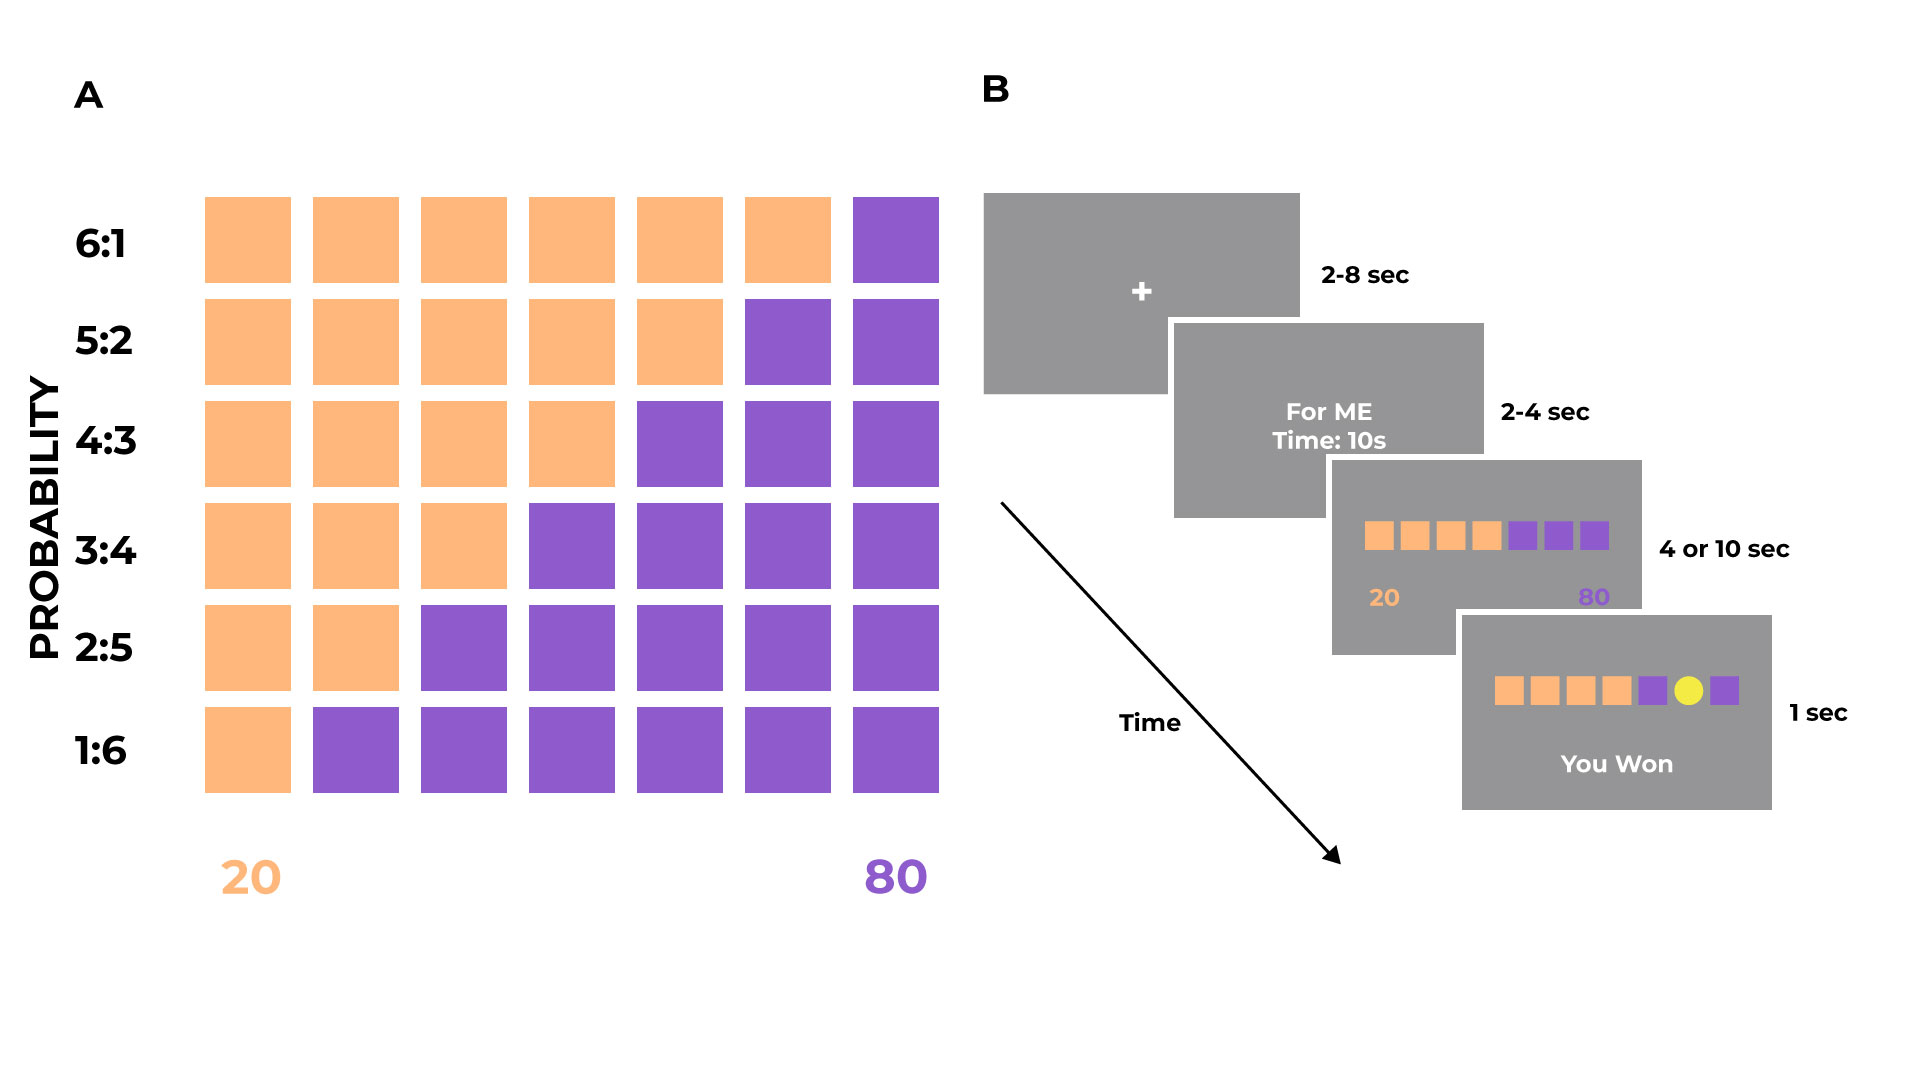
\includegraphics[scale=0.2]{figures/paradigm.jpg}
    \caption{Schematic of the frame-by-frame paradigm. A: The six experimental condtions with variable winning odds and fixed outcomes. B: The experimental design. Each trial began with a fixation followed by a cue screen where they were instructed about their choice and time limit. This was followed by the next screen where they had to play the gambling game and press a button to make their choice. The final screen showed whether they won or lost.}
    \label{fig:1}
\end{figure}
\subsection{Acquisition}
Functional images were acquired by T2*-weighted gradient-echo echo- planar imaging (35 slices, flip angle = 75 degree, time repetition [TR] = 2000 ms, time echo [TE] = 30 ms, voxel size 3 x 3 x 4 mm) on a 3T MRI scanner (Tim Trio, Siemens). Anatomical images were acquired using a T1-weighted MPRAGE sequence (176 slices, flip angle = 9 degree,TR = 2300 ms, TE = 2.98 ms, FOV 256, voxel size 1.0 x 1.0 x 1.1 mm). We used BrainVoyager QX 2.0.8 (Brain Innovation) for image pre-processing (slice scan time correction, 3D motion correction, high-pass filter with 2 cycles/experiment, normalization to Talairach stereotactic space (\cite{talairach1988co}), spatial smoothing with an isotropic Gaussian kernel of 6 and 8 mm full-width- half-maximum for single subject and group analyses, respectively) and estimation of statistical maps using a general linear model approach (\citet{friston1994functional}) with 6 rigid-body realignment parameters as nuisance covariates.(Parameters were adopted from \citet{hesselmann2011link}. 

\subsection{fMRI Data Analyses}
The data was later processed  and analyzed using Statistical Parametric Mapping 12 (SPM12; the Wellcome Trust Centre for Neuroimaging, University College London, UK). The statistical group maps were corrected for multiple comparisons using false discovery rate (FDR) control (Benjamini and Hochberg 1995; Genovese et al. 2002) and projected on the inflated and flattened cortical surface of one representative subject.

In order to explore which brain regions were activated when the decisions were made for self in contrast to when it was made on behalf of others, the whole brain contrast maps were estimated during the period when they were staring at the screen when the trial was on and received reward for their decision. 

\subsubsection{Trial related BOLD activation}
In order to model the different events in the task, 5 regressors were used in the model. (1) Decision events at the onset of the task. (2) Button Presses (3) Feedback events, when they came to know if they won or lost (4) Missed trials (5) Motion parameters. The group level activation map was obtained by performing a one-sample t-test over the individual subject contrast maps (random-effects modeling). This group level activation map was false discovery rate (FDR) corrected (P < 0.05) to account for multiple comparisons. 


% --------------------
\section{Results}
\subsection{Behavioural Results}
The ratio of risky choices to the total number of trials was calculated for each participant. Since the assumption of sphericity was violated according to Mauchly's test, we conducted multivariate tests. We conducted a 2(decision- self and decision- others for more time) x 6(Winning odds of the high risk option) ANOVA and it revealed a significant two way interaction effect [F(5,20) = 3.1741, p < 0.05]. Next we conducted the similar analysis for the case of less time [F(5,20) = 4.1, p > 0.05] and it did not reveal any significant difference between the two decision conditons. Next, we conducted a 2 (Decision for Self in More time and less time) x 6(Winning odds of the high risk option) ANOVA and it revealed a significant two way interaction effect [F(5,20) = 2.9982, p < 0.05]. Similarly, the same ANOVA was conducted for the decision made on behalf of others and it also revealed a significant two-way interaction effect [F(5,20) = 3.0012, p < 0.05]. Participants were more likely to make risky decisions for self than for others when the winning probability was higher. Moreover, the time constraint played a significant role. Indeed, more time led them to deliberately make their decision and thus choose less risky options throughout the task. (Figure 2)

\begin{figure}[H]
    \centering
        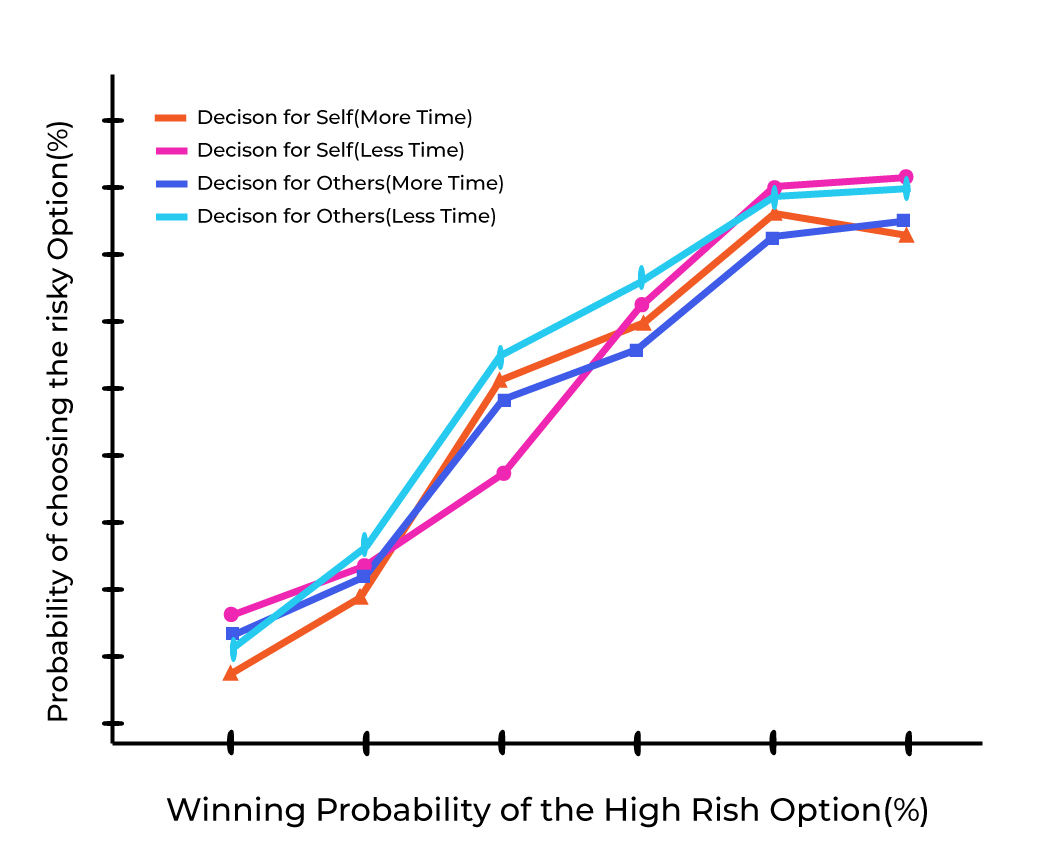
\includegraphics[scale=0.4]{figures/behav.jpg}
    \caption{ Behavioural data showing the probability of risky choice as a function of the potential outcome of the high risk option.}
    \label{fig:2}
\end{figure}

\subsection{Neuroimaging Results}
We used small- volume corrections (SVC) method for multiple comparisons( p< 0.05) in SPM12 The volumes for SVC were contained to spheres with radii of 15mm the center coordinates were utilized from previous studies. We applied a less stringent significance level(p < 0.001) in order to reduce the risk of false negatives and outline the clusters at which the activation have occurred. 

Brodmann areas and brain regions were pointed out in Talairach space (\citet{talairach1988co})  after converting the MNI coordinates to Talairach ones using non- linear transformation (\citet{lancaster2007bias}). 

In order to compare the brain regions activated when the person makes decision for oneself in contrast to when made for another, the contrasts were made at the time of decision or the task onset time. It was also found that both the cases of decision making activated the left intraparietal sulcus(IPS) (x = -27, y = -55,z= 56) and the decisions for the self activated the right IPS also (x = 31, y = -55, z= 55) (Figure 3 (a)). The decisions made for oneself elicited greater activity in the amygdala than what was observed for when the decisions were made on behalf of others which is associated with emotion processing (Figure 3 (b)). Further, it was observed that during the decisions for self, when they were given more time, the temporo - parietal cortex(TPC) elicited a greater response than when they were given less time to make their decision(Figure 3 (c)). Moreover the dmPFC activity exhibited a value difference and showed opposite activation in both cases when they made decision for self and others. Also, when the subject was making decisions on the behalf of others, we observed activation is some areas belonging to the Default Mode Network(Temporo parietal junction(TPJ, Insula, PCC) which corroborates the recruitment of the DMN when someone is thinking about others(Figure 3(d)). Finally, we observed some activation in the Anterior Singulate Cortex(ACC) (x = 4, y = 24,z= 40)(Figure 3 (e)) when the subject was given less time to make a decision for self and others and it was modulated by the decision towards choosing the risky option.

\begin{figure}
\centering
  \begin{subfigure}[b]{0.4\textwidth}
    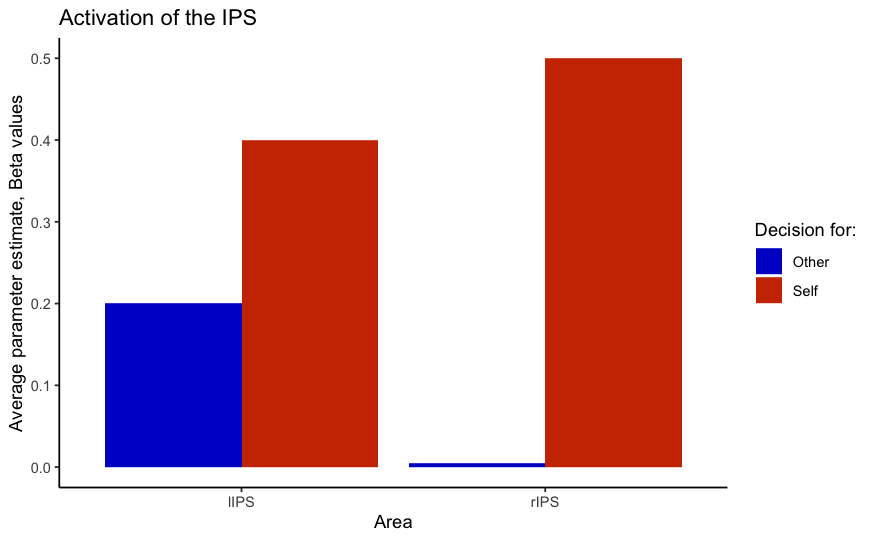
\includegraphics[width=\textwidth]{figures/IPS.png}
    \caption{Activation of the left and right IPS}
    \label{fig:3a}
  \end{subfigure}
  %
  \begin{subfigure}[b]{0.4\textwidth}
    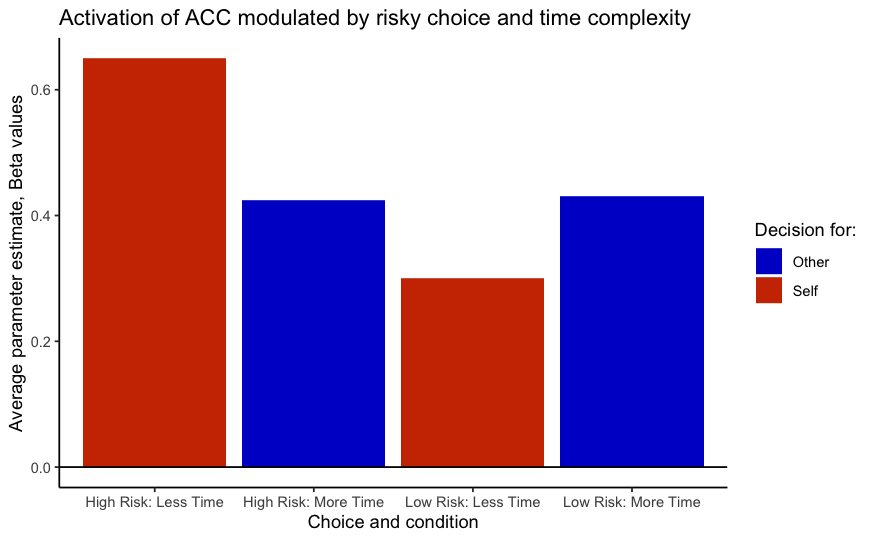
\includegraphics[width=\textwidth]{figures/acc.png}
    \caption{Activation of amygdala}
    \label{fig:3b}
  \end{subfigure}\\
  %
  \begin{subfigure}[b]{0.4\textwidth}
    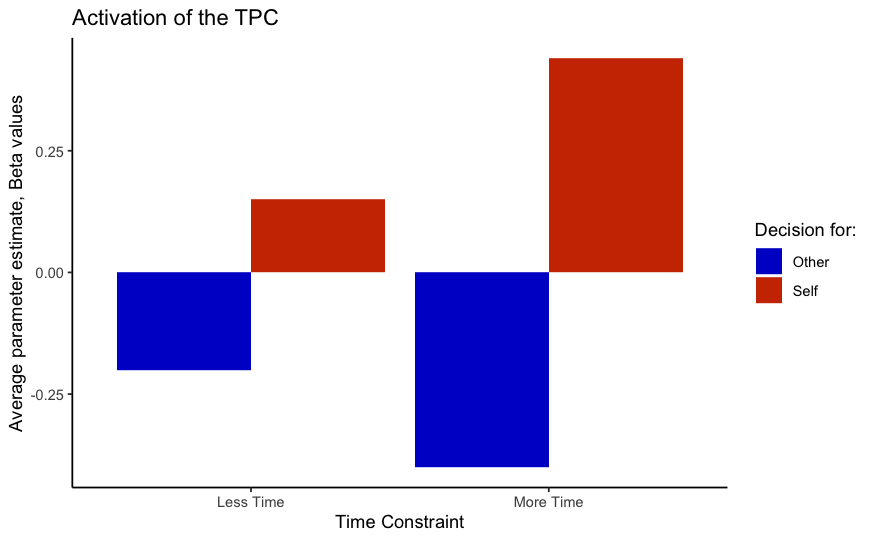
\includegraphics[width=\textwidth]{figures/tpc.png}
    \caption{Activation of TPC                    }
    \label{fig:3c}
  \end{subfigure}
  %
  \begin{subfigure}[b]{0.4\textwidth}
    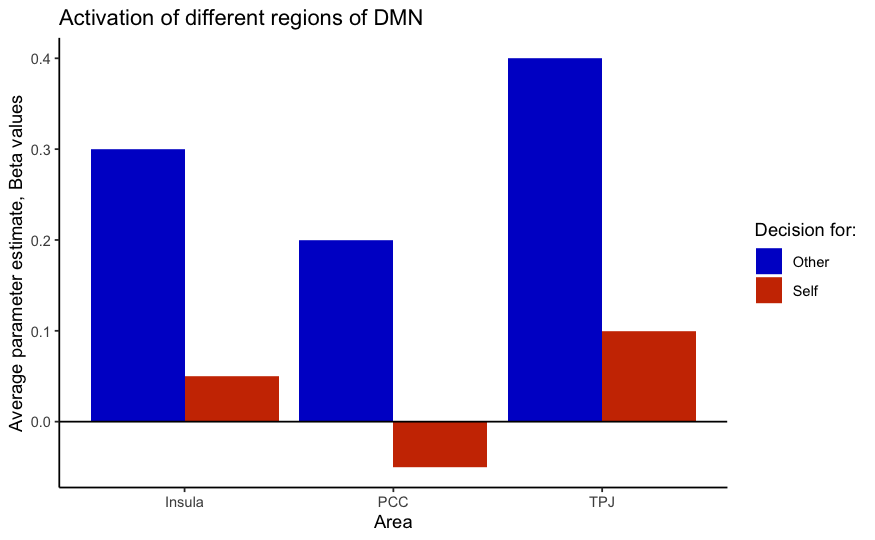
\includegraphics[width=\textwidth]{figures/dmn.png}
    \caption{Activation of diff. areas of DMN}
    \label{fig:3d}
  \end{subfigure}\\
  %
  \begin{subfigure}[b]{0.4\textwidth}
    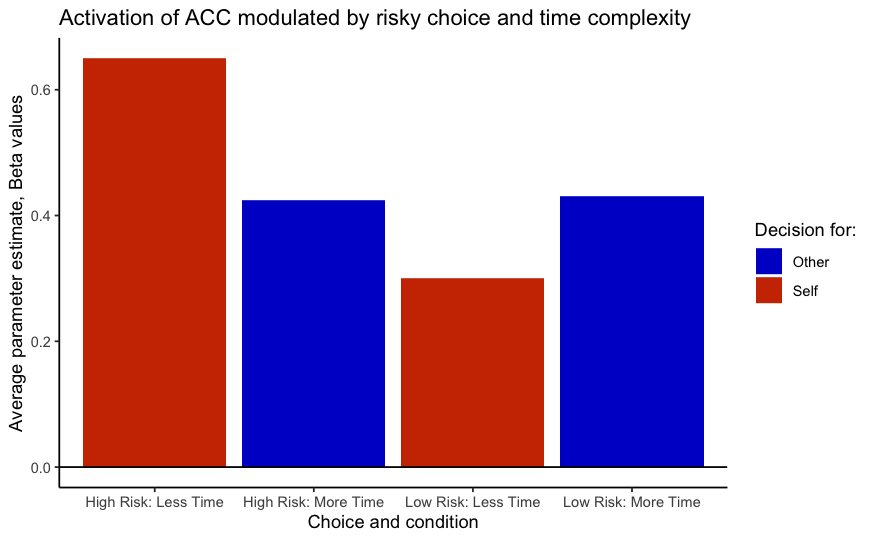
\includegraphics[width=\textwidth]{figures/acc.png}
    \caption{Activation of the anterior singulate cortex(ACC)}
    \label{fig:3e}
  \end{subfigure}
  \caption{Barplots describing the different activation parts in the different parts of the brain when the subject is making a decision on behalf of self and other and also how it is modulated by the two time constraint.}
    
\end{figure}


% --------------------
\section{Discussion and Conclusions}
% --------------------
The neural underpinning of social decision making were investigated by analysing the fMRI data that was collected. We found that different areas of the brain get activated at a different level when the subject is making a decision based on self vs. when the decision is made on the behalf of someone else. We observed changes in different activation with the modulation of cognitive, social and environmental factors. The amygdala was activated in both situations of decision making for self and the other but we observed an increased activation when the time given to make a decision was less. This can be explained by increased information processing per se emotions and risk as to make the choice as early as possible weighing in the other factors like risk (\citet{ghods2009fundamental}; \citet{smith2009neural}; \citet{morrison2010re}). We further observed activations in the dmPFC which can be associated with value computations for decisions on behalf of oneslef and others(\citet{cohen2005functional}). This can be attributed to the precise computational functions during social learning (\citet{behrens2008associative};\citet{behrens2009computation}; \citet{hampton2008neural}). One of the simplest explanation of this effect can be that the region is simulating one's own, relevant and irrelevant preferences and and also alternatively processing one's own translation of preference and relevance to the other partner's perspective. Activation in the ACC reflected the involvement in reward anticipation and feedback during the risky choice (\citet{ernst2004choice}) and in our study it reflected the anticipation of the winning or losing when the decision was being made. 

\medskip

\bibliography{references.bib} 

\end{document}